\documentclass[11pt]{article}
\usepackage[margin=1.05in]{geometry}
\usepackage{amsmath,amssymb,amsthm}
\usepackage{booktabs}
\usepackage{array}
\usepackage{tabularx}
\usepackage[protrusion=true,expansion=false]{microtype}
\usepackage[table]{xcolor}
\usepackage{enumitem}
\usepackage{titlesec}
\usepackage{float}
\usepackage{tikz}
\usetikzlibrary{arrows.meta,positioning,calc,backgrounds}
\usepackage{hyperref}

\hypersetup{colorlinks=true, linkcolor=blue!60!black, urlcolor=blue!60!black, citecolor=blue!60!black}
\usepackage[skip=0.6\baselineskip, indent=0pt]{parskip}

\titleformat{\section}{\large\bfseries}{\thesection.}{0.7em}{}
\titleformat{\subsection}{\normalsize\bfseries}{\thesubsection.}{0.6em}{}

\theoremstyle{plain}
\newtheorem{proposition}{Proposition}
\theoremstyle{definition}
\newtheorem{definition}{Definition}

% ----- notation -----
\newcommand{\vmax}{V_{\max}}
\newcommand{\Tc}{T_{\mathrm{close}}}
\newcommand{\bcorr}{b_{\mathrm{corr}}}
\newcommand{\tx}[1]{\texttt{#1}}
\newcommand{\cat}{\,\|\,}
\newcommand{\be}[2]{\langle #1\rangle_{#2}}          % big-endian encoding
\newcommand{\pre}[1]{[#1]_8}                         % first 8 bytes
\newcommand{\xo}[1]{\mathsf{x}(#1)}                  % x-only
\newcommand{\Ht}[1]{H_{\textsf{#1}}}                 % our tagged hash
\newcommand{\Hb}[1]{H^{340}_{\textsf{#1}}}           % BIP340 tagged hash
\newcommand{\Sign}{\mathsf{Sign}}
\newcommand{\Vfy}{\mathsf{Verify}}
\newcommand{\PSign}{\mathsf{PreSign}}
\newcommand{\PVfy}{\mathsf{PreVerify}}
\newcommand{\Compl}{\mathsf{Complete}}
\newcommand{\Extr}{\mathsf{Extract}}
\newcommand{\Wots}{\mathsf{W}}
\newcommand{\kiss}{k_{\mathrm{iss}}}
\newcommand{\sid}{\mathit{sid}}
\newcommand{\owed}{\mathsf{owed}}
\newcommand{\enc}{\mathsf{enc}}
\newcommand{\PH}{P_H^{c}}
\newcommand{\dH}{d_H^{c}}
\newcommand{\Oc}{O_c}

\newcolumntype{L}{>{\raggedright\arraybackslash}X}
\renewcommand{\arraystretch}{1.3}
\makeatletter
\setlength{\@fptop}{0pt}
\setlength{\@fpsep}{1.5\baselineskip}
\setlength{\@fpbot}{0pt plus 1fil}
\makeatother

\newenvironment{algobox}[1]
  {\par\smallskip\noindent\begin{tabular}{|p{0.955\linewidth}|}\hline\textbf{#1}\\[2pt]}
  {\\\hline\end{tabular}\par\smallskip}

\title{\textbf{The grants L2}\\a Lichen L2 without global order\\[2pt]\large early draft}
\author{waxwing}
\date{Version 0.1, November 2026\\[2pt]\small a companion to \emph{Lichen}, version 0.5~\cite{lichen}}

\begin{document}
\maketitle

\begin{abstract}
Lichen~\cite{lichen} enforces an L2's withdrawals through bilateral
contracts between a hub and each user, settled on Bitcoin by BABE with
the roles swapped: the user claims, and only the hub proves, if it can,
that she is owed less. This draft describes a second L2 for those
contracts, with no sequencer, no global ordering and no anchoring. Notes
are transparent and signed by the hub. A payment is made atomic by a
\emph{grant}: adaptor pre-signatures under a one-time point $T$ that the
hub opens only after the payer has signed, as in the ecash design
of~\cite{ecash} without the blinding. An exit posts a compact claim of
the user's notes, one-time signed in full. The hub answers a claim it
can show is too high by posting $\bcorr$, what she is owed, and proving
it from spends she signed. A spend counts against her only if the hub
reveals its unlock to her on chain, which it can do only by completing,
in its own transaction, a pre-signature she checked before paying. This
version spells out every object and step with explicit notation; it is
written to pin the algorithm down, not to be short.
\end{abstract}

\tableofcontents

\section{Setting}

A Lichen contract (\cite{lichen}, \S3) locks the hub's liquidity and the
user's deposit in one Bitcoin output, with a cap $\vmax$, a unit $u$ in
sats ($b$, an amount in units, is a 4-byte word), reserves $r_A$ (hers)
and $r_H$ (the hub's), and a close time $\Tc$. It ends in one of three
ways:
\begin{itemize}[nosep]
\item \textbf{Fold}: both sign; the user is paid what she withdraws and
  her reserve.
\item \textbf{Default}: after $\Tc$, the user is paid $r_A$ and the hub
  the rest. She must withdraw or exit before.
\item \textbf{Exit}: the user posts \tx{request} with a claim of $b$
  units; the hub either lets it pay or proves her owed less.
\end{itemize}

The anchored L2 (the reference L2 of~\cite{lichen}) judges a claim
against a global, anchored history. The grants L2 drops that: the hub's
book is the only ledger, and nothing is ordered beyond what each spend
names. What replaces the history is \emph{evidence the user signed}: a
claim is reduced only by spends she authorized and whose unlock the hub
gave her, on chain if not before.

\textbf{Contracts and credit.} A user's participation is defined by her
contract. Each contract $c$ has an L2 key $\Oc$ of its own, fresh at the
opening; the notes owned by $\Oc$ are what $c$'s exit can claim. Notes
owned by any other key (a wallet with no contract, a closed contract's
key) are the hub's IOUs with no backing on chain: credit. A wallet moves
its notes to its open contract's key with an ordinary payment to itself.

\section{Notation}\label{sec:notation}

\subsection{Group, encodings, hashes}

\begin{itemize}[nosep]
\item secp256k1: generator $G$, group order $n$. Lower-case letters are
  scalars mod $n$, upper-case letters are points.
\item $\xo{P}$: the 32-byte x-coordinate of $P$. $\mathsf{lift}(x)$: the
  point with x-coordinate $x$ and even $y$ (BIP340's \textsf{lift\_x}).
  $P^{(33)}$: $P$ compressed (33 bytes).
\item Every public key is x-only (BIP340~\cite{bip340}): a key pair
  $(d, P)$ has $P = dG$ with even $y$, $d$ negated if needed. Keys are
  written as points but encoded as $\xo{P}$.
\item $\be{v}{k}$: $v$ as $k$ bytes, big-endian. $\pre{h}$: the first 8
  bytes of $h$. $\cat$: concatenation.
\item $\Ht{tag}(p_1, \dots, p_r)$, the L2's tagged hash, is
  \[
    \mathrm{SHA256}\big(\textsf{tag} \cat \texttt{0x00} \cat \be{|p_1|}{4}
    \cat p_1 \cat \cdots \cat \be{|p_r|}{4} \cat p_r\big),
  \]
  with tags \textsf{lichen/notes/note}, \textsf{/spend}, \textsf{/out},
  \textsf{/grant}, \textsf{/grant-commitment}, \textsf{/auth},
  \textsf{/unlock}, \textsf{/issue}, \textsf{/half-agg}, written
  $\Ht{note}, \Ht{spend}, \dots$ below. Every part is length-prefixed,
  so no two different part lists hash alike.
\item $\Hb{tag}(x) = \mathrm{SHA256}(\mathrm{SHA256}(\textsf{tag}) \cat
  \mathrm{SHA256}(\textsf{tag}) \cat x)$, BIP340's tagged hash, and the
  challenge
  \[
    e(R, P, m) = \Hb{BIP0340/challenge}\big(\xo{R} \cat \xo{P} \cat m\big) \bmod n.
  \]
  It depends on $R$ only through $\xo{R}$.
\end{itemize}

\subsection{Signatures and adaptor signatures}

\textbf{BIP340.} $\Sign_d(m) = (r, s)$ with $r = \xo{R}$, $R = kG$ of
even $y$, $s = k + e(R, P, m)\,d$. $\Vfy_P(m, (r, s))$ holds iff $\hat R
= sG - e(\mathsf{lift}(r), P, m)P$ has even $y$ and $\xo{\hat R} = r$;
equivalently, $sG = \mathsf{lift}(r) + eP$. A signature is 64 bytes.

\textbf{Adaptor signatures} under a point $T$ (\tx{lngap\_btc::adaptor}):
\begin{itemize}[nosep]
\item $\PSign_d(m, T) = \mu = (r, R', s')$: pick a nonce $k$
  (deterministically, from $d$, $m$, $T$ and a counter), $R' = kG$, $R
  = R' + T$; retry with the next counter until $R$ has even $y$. Then
  $r = \xo{R}$ and $s' = k + e(R, P, m)\,d$.
\item $\PVfy_P(m, T, \mu)$ holds iff $R' + T$ has even $y$, $\xo{R' + T} =
  r$, and $s'G = R' + e(\mathsf{lift}(r), P, m)P$.
\item $\Compl(\mu, t) = (r, s' + t)$, a BIP340 signature by $P$ on $m$
  when $tG = T$: $(s' + t)G = R' + eP + T = R + eP$.
\item $\Extr(\mu, (r, s)) = s - s'$.
\item $\enc(\mu) = r \cat R'^{(33)} \cat \be{s'}{32}$: 97 bytes. The
  \emph{final nonce} of $\mu$ is $r$, its first 32 bytes.
\end{itemize}

\textbf{One-time signatures.} $\Wots_K(x)$ is a Winternitz signature
under the one-time key $K$ on the bytes $x$: 2 digits a byte, plus
checksum digits, 2 witness items per digit (a hash preimage and the
digit). Tapscript verifies it digit by digit, so the digits on the
stack are authenticated by Bitcoin itself. A key fixed in a leaf at the
opening signs once.

\subsection{Keys}

\begin{center}
\begin{tabularx}{\linewidth}{llL}
\toprule
Symbol & Scope & Use \\
\midrule
$\kiss$, $I = \kiss G$ & the deployment (one) & the issuer key: signs every note and every grant's $T$; pre-signs the outputs of every grant \\
$\dH$, $\PH$ & contract $c$ & the hub's payment key in $c$: its half of the 2-of-2 on every link of $c$'s graph; the key of \tx{correct}'s slots; signs the reveals for $c$ \\
$a_c$, $\Oc = a_c G$ & contract $c$ & her L2 key, fresh for $c$: owns the notes $c$'s exit claims; signs her spends of them. Called the \emph{owner} of $c$ \\
$P_A^c$ & contract $c$ & her half of the 2-of-2 \\
$K_b^c$, $K_P^c$ & contract $c$ & her one-time keys for $b$ and for the posted claim (in \tx{request}'s leaf) \\
$K_{\mathrm{corr}}^c$ & contract $c$ & the hub's one-time key for $\bcorr$ (in \tx{correct}'s leaf) \\
$t_S$, $T_S = t_S G$ & spend $S$ & the spend's unlock, derived by the hub \\
$t_0$, $T_0 = t_0G$ & the opening of $c$ & the unlock of the deposit's note (the mint) \\
\bottomrule
\end{tabularx}
\end{center}

The hub derives each contract's keys from its seed and $c$; it derives
$\kiss$ once. So $I$ is common to every contract, while $\PH$ differs per
contract: a pre-signature under $\PH$ is good only in contract $c$.

\section{Notes, spends and grants}

\subsection{Notes}

\begin{definition}
A \emph{note} is $N = (\mathit{id}, o, v)$: a 32-byte id, an owner (an
x-only key) and a value in sats ($v < 2^{48}$ for a claim). Its short id
is $\iota = \pre{\mathit{id}}$, and its digest
\[
  \delta(N) = \Ht{note}\big(\pre{\mathit{id}},\ o,\ \be{v}{8}\big).
\]
$N$ is \emph{settled} when its holder has $\sigma_N$ with
$\Vfy_I(\delta(N), \sigma_N)$.
\end{definition}

The digest names the note by its short id, so a claim on chain can name
it in 8 bytes (\S\ref{sec:claim}). The book keys notes by the full id.
Two notes of one owner with the same short id and value would share
their signature; only the owner can grind for that ($2^{32}$ spends of
hers), and it only harms her.

\subsection{Spends}

\begin{definition}
A \emph{spend} $S = (N_1, \dots, N_m;\ (o'_0, v'_0), \dots, (o'_{k-1},
v'_{k-1}))$ names input notes and asks for outputs. It is well formed if
$1 \le m \le 16$, $1 \le k \le 16$, the inputs are distinct, every $v'_j
> 0$, the $o'_j$ are distinct (one output per owner), and $\sum_i v_i =
\sum_j v'_j$. Its id is
\[
  \sid = \Ht{spend}\big(\be{m}{4},\ \delta(N_1), \dots, \delta(N_m),\
  \be{k}{4},\ o'_0 \cat \be{v'_0}{8}, \dots, o'_{k-1} \cat \be{v'_{k-1}}{8}\big),
\]
and its output notes are $N'_j = (\Ht{out}(\sid, \be{j}{4}),\ o'_j,\ v'_j)$
for $j = 0, \dots, k-1$.
\end{definition}

So a spend fixes the notes it makes. The rule of one output per owner
is the hub's (it refuses others); \S\ref{sec:volume} needs it.

\subsection{Grants}\label{sec:grant}

\begin{definition}
The hub's \emph{grant} on a well-formed spend $S$ whose inputs are live
(issued, unspent) is
\[
  \Gamma = \big(\sid,\ T_S,\ \tau,\ (\rho_j)_{j<k},\ ((o, \mu_o))_{o \in
  \mathcal{O}}\big),
\]
where
\begin{align*}
  t_S &= \Ht{unlock}(\kiss, \sid, \be{\mathit{ctr}}{4}) \text{ for the
  least } \mathit{ctr} \text{ giving } 0 < t_S < n, \qquad T_S = t_SG,\\
  \tau &= \Sign_{\kiss}\big(\Ht{grant}(\sid, T_S^{(33)})\big),\\
  \rho_j &= \PSign_{\kiss}\big(\delta(N'_j), T_S\big)\quad \text{for each output},\\
  \mu_o &= \PSign_{d_H^{c(o)}}\big(m_{c(o)}, T_S\big)\quad \text{for each } o \in \mathcal{O},
\end{align*}
$\mathcal{O}$ being the distinct input owners that are the owner of an
open contract $c(o)$, and $m_{c}$ that contract's \tx{correct} sighash
(\S\ref{sec:mc}). $(o, \mu_o)$ is $o$'s \emph{reveal}. The grant's
\emph{commitment} and the message the inputs' owners sign are
\begin{align*}
  C &= \Ht{grant-commitment}\big(\sid,\ T_S^{(33)},\ \be{k}{4},\
  \enc(\rho_0), \dots, \enc(\rho_{k-1}),\ o_1, \enc(\mu_{o_1}), \dots\big),\\
  \alpha &= \Ht{auth}(\sid, C).
\end{align*}
\end{definition}

$t_S$ is a function of the hub's key and the spend, so a spend asked
again gets the same grant. $\tau$ signs $\sid$ and $T_S$ together: it
binds this $T_S$ to this spend, so the payer can't choose $T_S$ (and
know $t_S$) herself, and the hub can't later show another one.

\subsection{A payment}\label{sec:payment}

Figure~\ref{fig:payment} shows a payment from Alice to Bob. Alice's
wallet spends all its notes (at most 16): the payment to Bob's address
$o_B$, and her change to her own address $o_A$ (her open contract's key
$\Oc$). Bob need not be online.

\begin{figure}[!tbp]
\centering
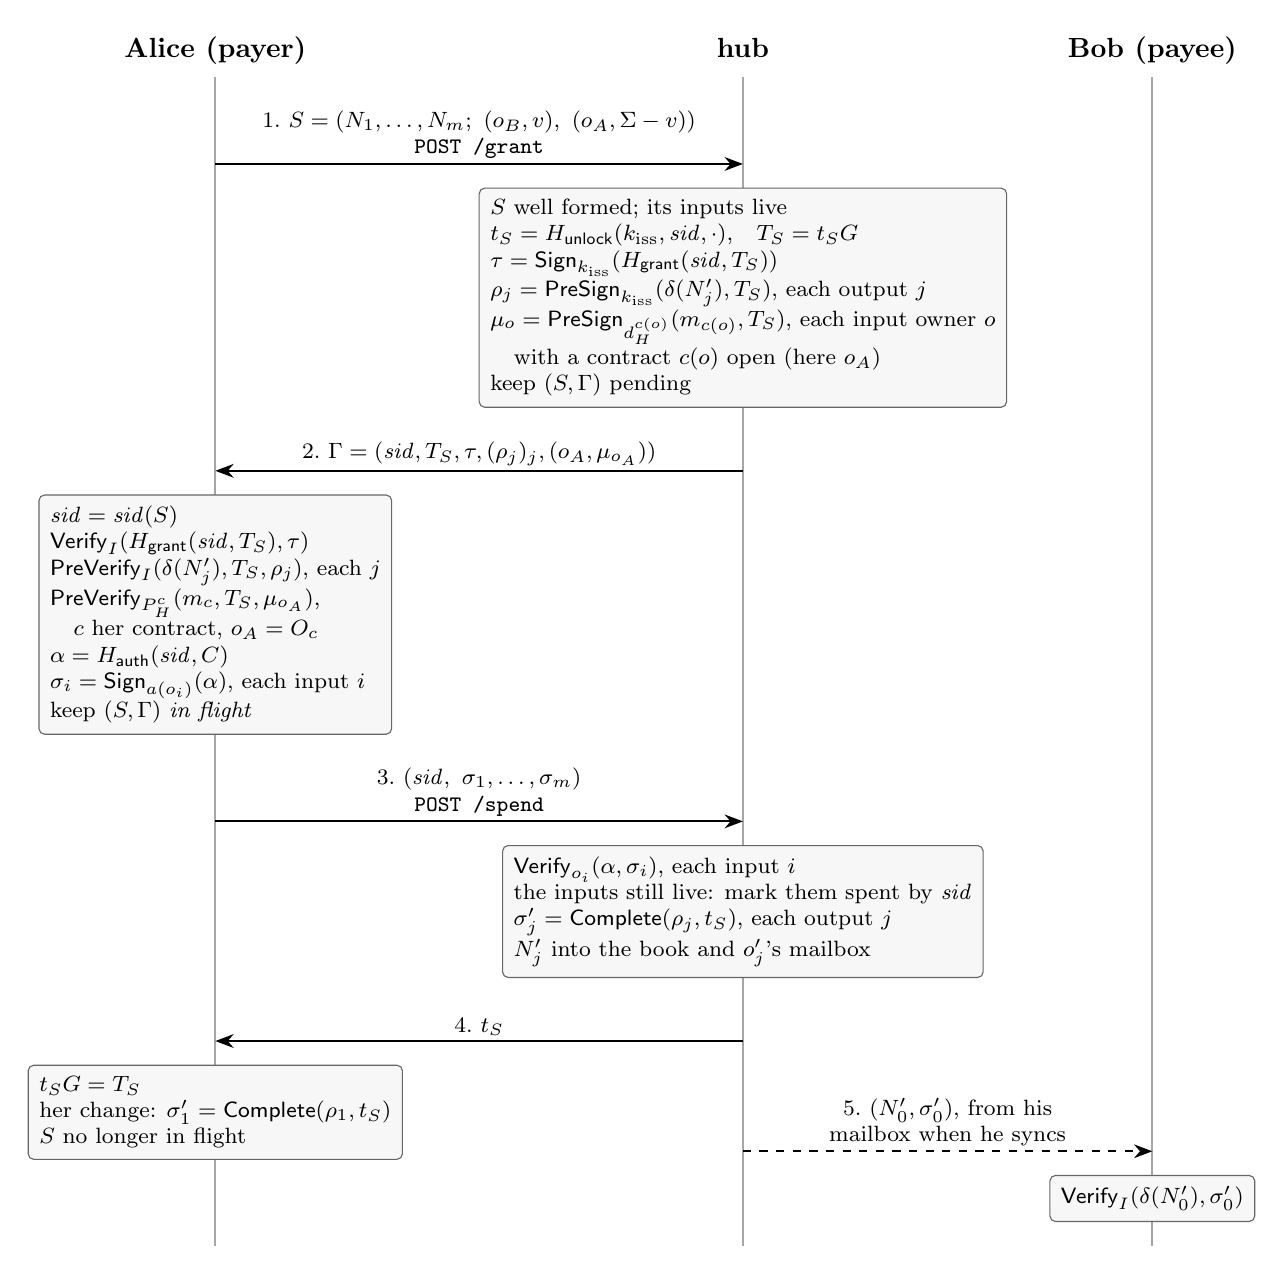
\begin{tikzpicture}[>=Stealth, font=\small,
  life/.style={draw=black!35, thick},
  box/.style={draw=black!60, fill=black!3, rounded corners=2pt, align=left, inner sep=4pt, font=\footnotesize},
  msg/.style={->, thick},
  lbl/.style={align=center, font=\footnotesize, inner sep=1.5pt}]
\coordinate (LA) at (2.6,0); \coordinate (LH) at (9.3,0); \coordinate (LB) at (14.5,0);
\node[font=\bfseries, anchor=base] at ($(LA)+(0,0.25)$) {Alice (payer)};
\node[font=\bfseries, anchor=base] at ($(LH)+(0,0.25)$) {hub};
\node[font=\bfseries, anchor=base] at ($(LB)+(0,0.25)$) {Bob (payee)};
% 1
\coordinate (y) at (0,-1.1);
\draw[msg] (LA|-y) -- node[lbl, above] {1.\ $S = (N_1, \dots, N_m;\ (o_B, v),\ (o_A, \Sigma - v))$\\ \tx{POST /grant}} (LH|-y);
\node[box, anchor=north] (b1) at ($(LH|-y)+(0,-0.3)$) {
  $S$ well formed; its inputs live\\
  $t_S = \Ht{unlock}(\kiss, \sid, \cdot)$,\quad $T_S = t_SG$\\
  $\tau = \Sign_{\kiss}(\Ht{grant}(\sid, T_S))$\\
  $\rho_j = \PSign_{\kiss}(\delta(N'_j), T_S)$, each output $j$\\
  $\mu_o = \PSign_{d_H^{c(o)}}(m_{c(o)}, T_S)$, each input owner $o$\\
  \quad with a contract $c(o)$ open (here $o_A$)\\
  keep $(S, \Gamma)$ pending};
% 2
\coordinate (y) at ($(b1.south)+(0,-0.8)$);
\draw[msg] (LH|-y) -- node[lbl, above] {2.\ $\Gamma = (\sid, T_S, \tau, (\rho_j)_j, (o_A, \mu_{o_A}))$} (LA|-y);
\node[box, anchor=north] (b2) at ($(LA|-y)+(0,-0.3)$) {
  $\sid = \sid(S)$\\
  $\Vfy_I(\Ht{grant}(\sid, T_S), \tau)$\\
  $\PVfy_I(\delta(N'_j), T_S, \rho_j)$, each $j$\\
  $\PVfy_{\PH}(m_c, T_S, \mu_{o_A})$,\\
  \quad $c$ her contract, $o_A = \Oc$\\
  $\alpha = \Ht{auth}(\sid, C)$\\
  $\sigma_i = \Sign_{a(o_i)}(\alpha)$, each input $i$\\
  keep $(S, \Gamma)$ \emph{in flight}};
% 3
\coordinate (y) at ($(b2.south)+(0,-1.1)$);
\draw[msg] (LA|-y) -- node[lbl, above] {3.\ $(\sid,\ \sigma_1, \dots, \sigma_m)$\\ \tx{POST /spend}} (LH|-y);
\node[box, anchor=north] (b3) at ($(LH|-y)+(0,-0.3)$) {
  $\Vfy_{o_i}(\alpha, \sigma_i)$, each input $i$\\
  the inputs still live: mark them spent by $\sid$\\
  $\sigma'_j = \Compl(\rho_j, t_S)$, each output $j$\\
  $N'_j$ into the book and $o'_j$'s mailbox};
% 4
\coordinate (y) at ($(b3.south)+(0,-0.8)$);
\draw[msg] (LH|-y) -- node[lbl, above] {4.\ $t_S$} (LA|-y);
\node[box, anchor=north] (b4) at ($(LA|-y)+(0,-0.3)$) {
  $t_SG = T_S$\\
  her change: $\sigma'_1 = \Compl(\rho_1, t_S)$\\
  $S$ no longer in flight};
% 5
\coordinate (y) at ($(y)+(0,-1.4)$);
\draw[msg, dashed] (LH|-y) -- node[lbl, above] {5.\ $(N'_0, \sigma'_0)$, from his\\ mailbox when he syncs} (LB|-y);
\node[box, anchor=north] (b5) at ($(LB|-y)+(0,-0.3)$) {$\Vfy_I(\delta(N'_0), \sigma'_0)$};
\coordinate (end) at ($(b5.south)+(0,-0.3)$);
\begin{scope}[on background layer]
\foreach \l in {LA,LH,LB} \draw[life] (\l) -- (\l|-end);
\end{scope}
\end{tikzpicture}
\caption{A granted payment. Output 0 pays Bob $v$; output 1 returns
Alice's change. Before step 4 only the hub knows $t_S$, so the outputs
are unusable; after it they are ordinary settled notes.}
\label{fig:payment}
\end{figure}

\textbf{What Alice's signature covers.} $\alpha$ commits to $S$ (through
$\sid$), to $T_S$, to every output pre-signature and to every reveal, in
the bytes she checked. A cited spend in an exit is checked against
exactly these bytes (\S\ref{sec:statement}).

\textbf{In flight.} From step 3 until she has $t_S$, Alice keeps $(S,
\Gamma)$ and her inputs. The hub may claim it never recorded $S$; she
can't tell. She keeps claiming her inputs, with $S$ as a \emph{fallback}
(\S\ref{sec:claim}): if the hub uses $S$ against that claim, it must
reveal $t_S$ (\S\ref{sec:reveal}), and her change counts instead.

\textbf{What atomicity means here.} Once Alice signs, the hub may record
$S$ or not.
\begin{itemize}[nosep]
\item Not recorded: $t_S$ is never released (the hub alone knows it), so
  the outputs never settle, and her inputs stay hers.
\item Recorded, $t_S$ given (to her, or to Bob's mailbox): both sides
  are paid.
\item Recorded, $t_S$ withheld from both: the hub holds her inputs and
  pays no one; Bob has nothing to deliver goods against. Her exit
  settles it: the hub can count $S$ against her claim only by putting
  $t_S$ on chain for her; she then completes $\sigma'_0$ and hands Bob
  his note. Otherwise $S$ doesn't count, and her claim is owed its
  inputs.
\end{itemize}

\subsection{The wallet's policy}

A payment spends all the wallet's notes, to the payee and one change
note back. The wallet merges (a payment to itself, at its address) once
it holds more than 2 notes, or any note under a key other than its
address. Its address is its open contract's key $\Oc$, or its base key
if it has none. It refuses to pay itself any other way.

\section{The contract}

\subsection{Opening}\label{sec:opening}

The opening follows~\cite{lichen}, with the user's deposit and her L2
balance swapped atomically (Figure~\ref{fig:opening}):
\begin{enumerate}[nosep]
\item Alice derives a fresh key $a_c$, $\Oc = a_cG$, and pays her
  deposit $v_D$ to a coin $O_D$: a 2-of-2 of hers and the hub's, or her
  refund alone after a timeout.
\item She asks for a contract with owner $\Oc$. The hub refuses any
  $\Oc$ it has seen before: the owner of a contract, or of any note,
  pending or issued. So $\Oc$ has no history before $c$.
\item The setup (\cite{lichen}): the statement fixed (its journal,
  \S\ref{sec:journal}), the BABE instances garbled by Alice and kept by
  the hub by cut-and-choose.
\item The hub's offer: the funding $F$, which spends $O_D$ and the hub's
  coins into the contract output; its pre-signatures on the graph; and
  the \emph{mint}, the note
  \[
    N_0 = \big(\Ht{issue}(\texttt{"mint"} \cat \be{c}{4} \cat
    \mathrm{txid}(F)),\ \Oc,\ v_0\big),
  \]
  $v_0$ her deposit less the opening's fee, pre-issued as $\rho_0 =
  \PSign_{\kiss}(\delta(N_0), T_0)$, with $t_0$ the hub's, fresh for
  this $F$.
\item Alice checks $\PVfy_I(\delta(N_0), T_0, \rho_0)$ and $v_0$, signs
  the graph, and pre-signs $F$'s spend of $O_D$ under the same point:
  $\mu_F = \PSign_{a_D}(m_F, T_0)$, with $a_D$ her key in $O_D$ and $m_F$
  that input's sighash.
\item The hub completes $\sigma_F = \Compl(\mu_F, t_0)$, adds its own
  signature and broadcasts $F$.
\item Alice reads $\sigma_F$ from $F$'s witness: $t_0 = \Extr(\mu_F,
  \sigma_F)$, $\sigma_0 = \Compl(\rho_0, t_0)$. $N_0$ is settled; the
  hub enters it in the book.
\end{enumerate}
If the hub never broadcasts $F$, nothing settles $N_0$ and Alice
refunds $O_D$ after its timeout. If $F$ confirms, $t_0$ is on chain
whether or not the hub answers.

\begin{figure}[!tbp]
\centering
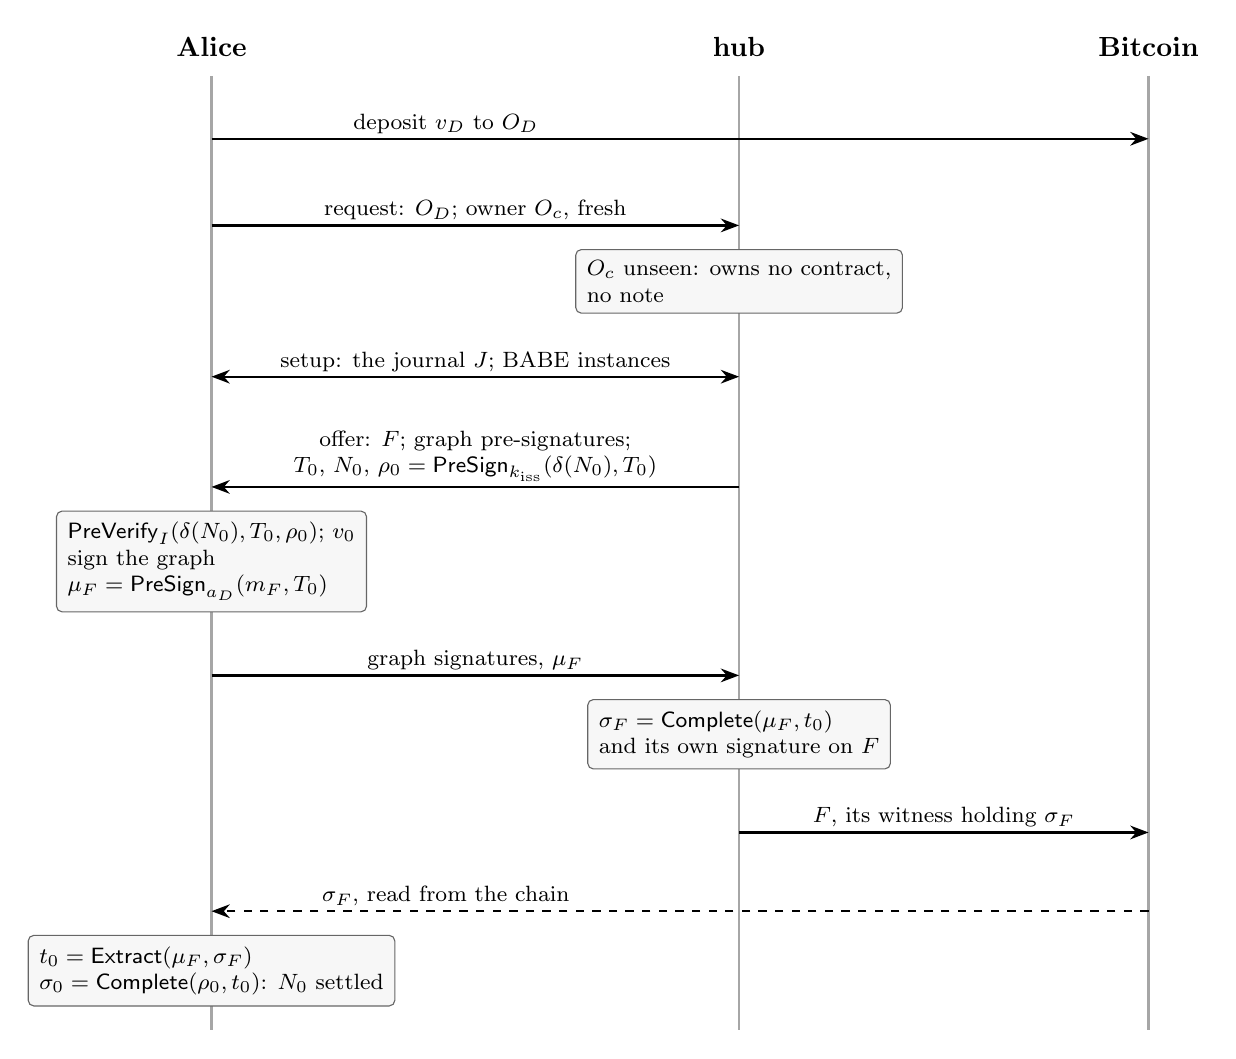
\begin{tikzpicture}[>=Stealth, font=\small,
  life/.style={draw=black!35, thick},
  box/.style={draw=black!60, fill=black!3, rounded corners=2pt, align=left, inner sep=4pt, font=\footnotesize},
  msg/.style={->, thick},
  lbl/.style={align=center, font=\footnotesize, inner sep=1.5pt}]
\coordinate (LA) at (2.6,0); \coordinate (LH) at (9.3,0); \coordinate (LB) at (14.5,0);
\node[font=\bfseries, anchor=base] at ($(LA)+(0,0.25)$) {Alice};
\node[font=\bfseries, anchor=base] at ($(LH)+(0,0.25)$) {hub};
\node[font=\bfseries, anchor=base] at ($(LB)+(0,0.25)$) {Bitcoin};
\coordinate (y) at (0,-0.8);
\draw[msg] (LA|-y) -- node[lbl, above, pos=0.25] {deposit $v_D$ to $O_D$} (LB|-y);
\coordinate (y) at ($(y)+(0,-1.1)$);
\draw[msg] (LA|-y) -- node[lbl, above] {request: $O_D$; owner $\Oc$, fresh} (LH|-y);
\node[box, anchor=north] (b1) at ($(LH|-y)+(0,-0.3)$) {$\Oc$ unseen: owns no contract,\\ no note};
\coordinate (y) at ($(b1.south)+(0,-0.8)$);
\draw[msg, <->] (LA|-y) -- node[lbl, above] {setup: the journal $J$; BABE instances} (LH|-y);
\coordinate (y) at ($(y)+(0,-1.4)$);
\draw[msg] (LH|-y) -- node[lbl, above] {offer: $F$; graph pre-signatures;\\ $T_0$, $N_0$, $\rho_0 = \PSign_{\kiss}(\delta(N_0), T_0)$} (LA|-y);
\node[box, anchor=north] (b2) at ($(LA|-y)+(0,-0.3)$) {$\PVfy_I(\delta(N_0), T_0, \rho_0)$; $v_0$\\ sign the graph\\ $\mu_F = \PSign_{a_D}(m_F, T_0)$};
\coordinate (y) at ($(b2.south)+(0,-0.8)$);
\draw[msg] (LA|-y) -- node[lbl, above] {graph signatures, $\mu_F$} (LH|-y);
\node[box, anchor=north] (b3) at ($(LH|-y)+(0,-0.3)$) {$\sigma_F = \Compl(\mu_F, t_0)$\\ and its own signature on $F$};
\coordinate (y) at ($(b3.south)+(0,-0.8)$);
\draw[msg] (LH|-y) -- node[lbl, above] {$F$, its witness holding $\sigma_F$} (LB|-y);
\coordinate (y) at ($(y)+(0,-1.0)$);
\draw[msg, dashed] (LB|-y) -- node[lbl, above, pos=0.75] {$\sigma_F$, read from the chain} (LA|-y);
\node[box, anchor=north] (b4) at ($(LA|-y)+(0,-0.3)$) {$t_0 = \Extr(\mu_F, \sigma_F)$\\ $\sigma_0 = \Compl(\rho_0, t_0)$: $N_0$ settled};
\coordinate (end) at ($(b4.south)+(0,-0.3)$);
\begin{scope}[on background layer]
\foreach \l in {LA,LH,LB} \draw[life] (\l) -- (\l|-end);
\end{scope}
\end{tikzpicture}
\caption{The opening: the deposit and the mint $N_0$ swap through one
adaptor point $T_0$.}
\label{fig:opening}
\end{figure}

\subsection{The journal}\label{sec:journal}

The statement's only public input, fixed at the opening, is the 68-byte
journal
\begin{align*}
  J &= \be{c}{4}^{\mathrm{LE}} \cat D \cat \mathrm{SHA256}(\texttt{"lichen/hp/contract"} \cat O_D \cat \be{\mathit{margin}}{4}),\\
  D &= \mathrm{SHA256}\big(\texttt{"lichen/contract"} \cat \Delta \cat 0^{36} \cat \be{W}{16} \cat [\be{u}{8}]\big),\\
  \Delta &= \mathrm{SHA256}(\texttt{"lngap/deployment"} \cat \xo{I} \cat \xo{\Oc}),
\end{align*}
with $c$ little-endian, $O_D$ the deposit coin (36 bytes), $0^{36}$ the
anchored L2's genesis seal (none here), $W$ the work the statement asks
on top of \tx{request}'s block (ten blocks' at the opening's
difficulty), and $\be{u}{8}$ present only if $u \ne 1$. \emph{margin}
is the anchored L2's and unused here. $D$ binds the issuer and the
owner: without the owner, a hub could prove against another key and
count every claim malformed.

\subsection{\tx{correct}'s sighash $m_c$}\label{sec:mc}

$m_c$ is the BIP341 signature hash of \tx{correct} (its one input,
spending \tx{request}'s output by the leaf \tx{correct}, with
\tx{SIGHASH\_DEFAULT} and no annex). \tx{correct} spends a pre-signed
chain whose transaction ids are fixed at the opening, and its outputs
are fixed too (fees come from an anchor output, by CPFP). So $m_c$ is
known at the opening, before any spend exists. The hub caches it per
contract and uses it for every reveal through $c$.

\subsection{The dispute graph}\label{sec:graph}

Every transaction has one input; every link has one output that carries
the value on, plus an anchor for fees. Each link is signed by the 2-of-2
$(P_A^c, \PH)$, pre-signed at the opening, and each output has its
terminal. Figure~\ref{fig:graph} shows the graph with each link's
poster, relative timelock and witness. $\epsilon$ is a short relative
lock on every link, so a link can't confirm in its parent's block.

\begin{figure}[!tbp]
\centering
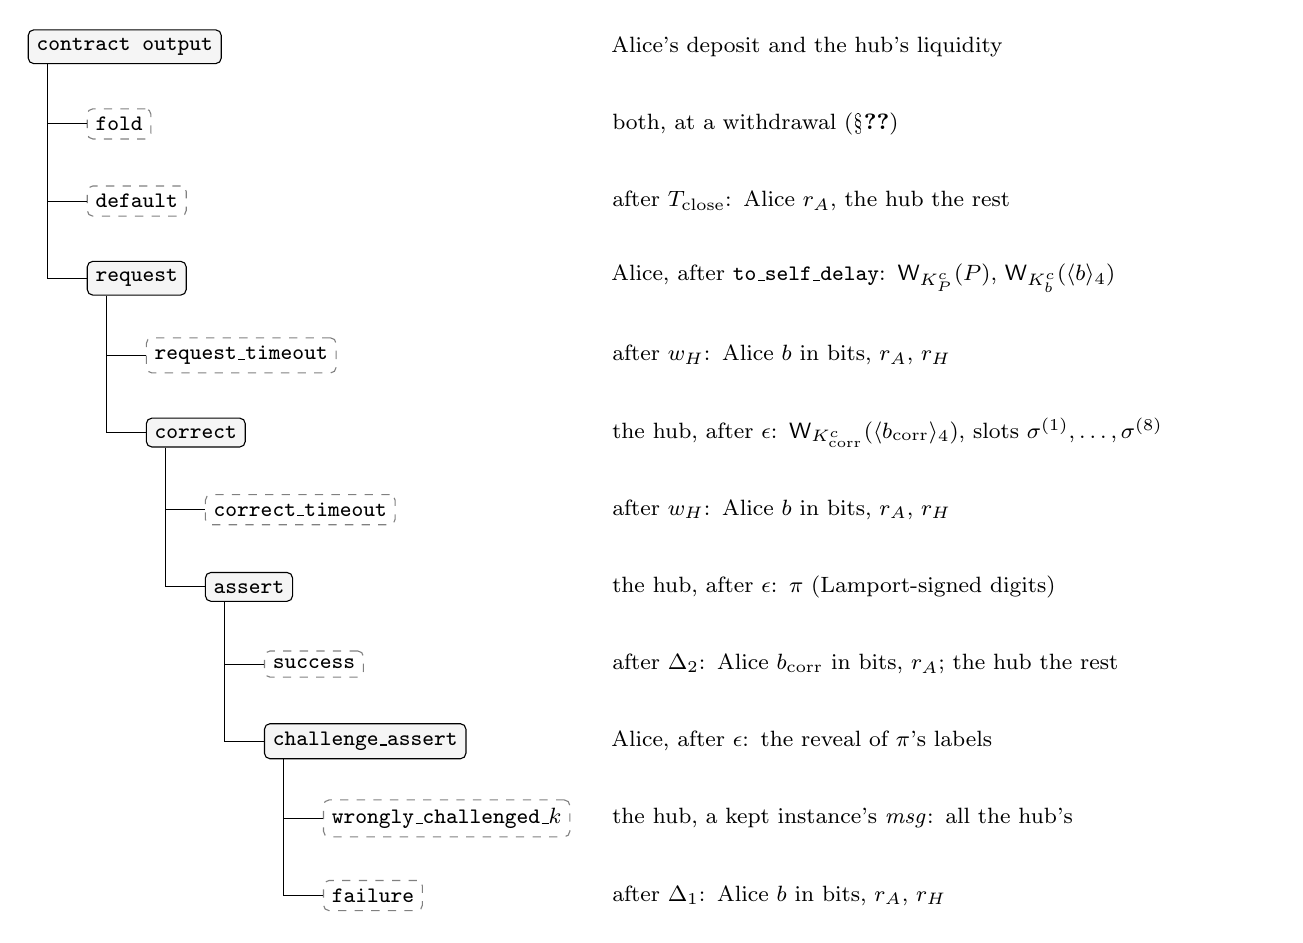
\begin{tikzpicture}[font=\footnotesize,
  link/.style={draw, rounded corners=2pt, inner sep=3pt, fill=black!4, font=\footnotesize\ttfamily, anchor=west},
  term/.style={draw=black!50, dashed, rounded corners=2pt, inner sep=3pt, font=\footnotesize\ttfamily, anchor=west},
  ann/.style={anchor=west, align=left, text width=8.3cm, font=\footnotesize}]
\def\dx{0.75}\def\dy{0.98}\def\ax{7.3}
\node[link] (c)  at (0*\dx, 0)      {contract output};
\node[term] (fo) at (1*\dx, -1*\dy) {fold};
\node[term] (de) at (1*\dx, -2*\dy) {default};
\node[link] (rq) at (1*\dx, -3*\dy) {request};
\node[term] (rt) at (2*\dx, -4*\dy) {request\_timeout};
\node[link] (co) at (2*\dx, -5*\dy) {correct};
\node[term] (ct) at (3*\dx, -6*\dy) {correct\_timeout};
\node[link] (as) at (3*\dx, -7*\dy) {assert};
\node[term] (su) at (4*\dx, -8*\dy) {success};
\node[link] (ch) at (4*\dx, -9*\dy) {challenge\_assert};
\node[term] (wc) at (5*\dx, -10*\dy){wrongly\_challenged\_$k$};
\node[term] (fa) at (5*\dx, -11*\dy){failure};
\foreach \p/\q in {c/fo,c/de,c/rq,rq/rt,rq/co,co/ct,co/as,as/su,as/ch,ch/wc,ch/fa}
  \draw ($(\p.south west)+(0.25,0)$) |- (\q.west);
\node[ann] at (\ax, 0)        {Alice's deposit and the hub's liquidity};
\node[ann] at (\ax, -1*\dy)   {both, at a withdrawal (\S\ref{sec:withdrawal})};
\node[ann] at (\ax, -2*\dy)   {after $\Tc$: Alice $r_A$, the hub the rest};
\node[ann] at (\ax, -3*\dy)   {Alice, after \tx{to\_self\_delay}: $\Wots_{K_P^c}(P)$, $\Wots_{K_b^c}(\be{b}{4})$};
\node[ann] at (\ax, -4*\dy)   {after $w_H$: Alice $b$ in bits, $r_A$, $r_H$};
\node[ann] at (\ax, -5*\dy)   {the hub, after $\epsilon$: $\Wots_{K_{\mathrm{corr}}^c}(\be{\bcorr}{4})$, slots $\sigma^{(1)}, \dots, \sigma^{(8)}$};
\node[ann] at (\ax, -6*\dy)   {after $w_H$: Alice $b$ in bits, $r_A$, $r_H$};
\node[ann] at (\ax, -7*\dy)   {the hub, after $\epsilon$: $\pi$ (Lamport-signed digits)};
\node[ann] at (\ax, -8*\dy)   {after $\Delta_2$: Alice $\bcorr$ in bits, $r_A$; the hub the rest};
\node[ann] at (\ax, -9*\dy)   {Alice, after $\epsilon$: the reveal of $\pi$'s labels};
\node[ann] at (\ax, -10*\dy)  {the hub, a kept instance's \textit{msg}: all the hub's};
\node[ann] at (\ax, -11*\dy)  {after $\Delta_1$: Alice $b$ in bits, $r_A$, $r_H$};
\end{tikzpicture}
\caption{A contract's graph. Solid boxes carry the value on, dashed ones
are terminals; every edge is a pre-signed spend of its parent's output.}
\label{fig:graph}
\end{figure}

\textbf{Bits.} A terminal pays an amount $x$ (in units) in binary: for
each bit position $i$ the contract has, an output of $u\,2^i$. In the
terminals that pay $b$, Alice spends output $i$ if bit $i$ of the $b$
she one-time signed in \tx{request} is set, the hub otherwise.
\tx{success} pays $\bcorr$ the same way, read from the hub's signature
under $K_{\mathrm{corr}}^c$ in \tx{correct}; a leaf \tx{equiv\_corr\_$i$} gives
Alice every bit output if she shows two different signatures under
$K_{\mathrm{corr}}^c$ (an equivocation).

\textbf{Windows} on Mutinynet (30\,s blocks): $w_H$ = 240 blocks (2
hours) for the hub to correct, and again to assert; $\Delta_2$ = 2,880
(a day) for her challenge; $\Delta_1$ = 240 for the hub's answer.

\textbf{No penalty.} \tx{success} returns her reserve whatever
$\bcorr$. A false claim gains her nothing (she is paid what she is
owed) and costs the hub one dispute; a penalty would also strike an
honest wallet restored from a stale backup.

\subsection{Withdrawal}\label{sec:withdrawal}

Alice hands the hub a full claim (\S\ref{sec:claim}) signed with $a_c$.
The hub takes it if it is owed in full by its book: it marks the notes
as taken by this contract's claim, issues their value beyond $bu$ back
to $\Oc$ as change (now credit), and both sign the fold. If the hub
takes the claim and won't fold, her exit posts the same claim; a claim
on the same contract never counts against itself.

\section{The exit}\label{sec:exit}

\subsection{The claim}\label{sec:claim}

\begin{definition}
A \emph{claim} on contract $c$ is $(b;\ N_1, \dots, N_n;\ \sid_1, \dots,
\sid_f)$ with $1 \le n \le 4$, $f \le 4$: settled notes of $\Oc$ with
distinct short ids, each with $\sigma_{N_i}$; $f$ \emph{fallbacks}, the
ids of her spends in flight that take any of the $N_i$, with distinct
$\pre{\sid_l}$; and $b \le \lfloor \sum_i v_i / u \rfloor$.
\end{definition}

The wallet picks the largest of $\Oc$'s notes that fit (below),
dropping the smallest until they do, and sets $b$ to what she
withdraws.

\textbf{The posted claim} $P$ is exactly 233 bytes:
\[
  P = \underbrace{\be{16n + f}{1}}_{\text{counts}} \cat
  \mathop{\Big\Vert}_{i=1}^{n} \big(\pre{\mathit{id}_i} \cat \be{v_i}{6} \cat r_i\big) \cat
  \underbrace{\be{s}{32}}_{\text{aggregate}} \cat
  \mathop{\Big\Vert}_{l=1}^{f} \pre{\sid_l} \cat 0^{\ast},
\]
where $\sigma_{N_i} = (r_i, s_i)$, $s$ is the half-aggregate below, and
$0^{\ast}$ pads with zeros to 233 bytes. It fits iff $1 + 46n + 32 + 8f
\le 233$ (with $1 \le n \le 4$, $f \le 4$): four notes and two
fallbacks, or three and four. The contract ($c$, $O_D$, $\Oc$) is not
in $P$: the statement takes it from the journal. $b$ is signed apart.

\textbf{Half-aggregation}~\cite{halfagg1,halfagg2}. Let $m_i =
\Ht{note}(\pre{\mathit{id}_i}, \Oc, \be{v_i}{8}) = \delta(N_i)$. With
weights
\[
  z_1 = 1,\qquad z_i = \Ht{half-agg}\big(\xo{I},\ r_1, m_1,\ \dots,\ r_i,
  m_i\big) \bmod n \quad (i \ge 2),
\]
the aggregate is $s = \sum_i z_i s_i$, and it verifies iff
\[
  sG = \sum_{i=1}^{n} z_i\big(\mathsf{lift}(r_i) + e(\mathsf{lift}(r_i),
  I, m_i)\,I\big).
\]
Alice computes $s$ from the signatures she holds. Each $z_i$ hashes
every $r$ and $m$ before it, so no signature can be traded for another.

\textbf{Signed in full.} \tx{request}'s witness carries
$\Wots_{K_P^c}(P)$ and $\Wots_{K_b^c}(\be{b}{4})$, so Bitcoin's script
checks every byte of $P$ and of $b$, and no one can swap them. A witness
item can't be bound any cheaper: tapscript has no \tx{OP\_CAT}, so a
hash computed in script can't be compared with signed digits. With the
2-of-2's signatures that makes 962 witness items, inside Bitcoin's 1,000
stack elements; that bounds $P$'s size.

\textbf{Why not shorter tags.} A MAC tag under a key the hub commits to
at the opening would be 8 bytes, but the user can't check it, so a hub
could issue bad tags and later call her notes unissued. A VRF output is
checkable and short, but the payee's tags would come from the hub after
$t_S$, outside the grant's atomicity. The hub's BIP340 signatures are
hers to check, and are released by $t_S$ with the outputs.

\subsection{The hub's answer}\label{sec:answer}

When \tx{request} confirms, the hub:
\begin{enumerate}[nosep]
\item reads $b$ and $P$ from \tx{request}'s witness, and maps each posted
  note $(\iota_i, v_i)$ to its book (owner $\Oc$) and each fallback
  $\pre{\sid_l}$ to a recorded spend;
\item gathers the evidence: for each claimed note the recorded spend
  that took it, and, through a spend the claim names as a fallback, that
  spend's output to $\Oc$ in turn;
\item computes $x = \owed(\cdot)$ (Algorithm~1) with the
  statement's own function, the evidence cited and its reveals' final
  nonces as the slots;
\item takes the claim into its book at $x$: its live notes (and revived
  change) are marked taken, so no later spend of them is recorded;
\item if $x = b$: does nothing; \tx{request\_timeout} pays her $b$;
\item otherwise posts \tx{correct} with $\bcorr = x$ and, in its slots,
  $\sigma^{(q)} = \Compl(\mu^{(q)}, t_{S_q})$ for each cited spend $S_q$
  ($\mu^{(q)}$ the reveal for $\Oc$ in $S_q$'s grant), the unused slots
  each a plain $\Sign_{\dH}(m_c)$;
\item once \tx{request}'s block carries $W$, checks the statement
  natively, proves it (about 21 minutes on a 4-core server), wraps it
  in Groth16, and posts \tx{assert}.
\end{enumerate}
After \tx{success} it sweeps the bit outputs that are its own once
their timelock has passed.

\textbf{\tx{correct}'s leaf} (all of it, with $\PH$ the same key as in
the 2-of-2):
\[
  \langle\text{2-of-2}\rangle\ \ \langle\Wots\text{-verify } K_{\mathrm{corr}}^c,
  \text{4 bytes}\rangle\ \ \big(\tx{OP\_SIZE}\ 64\ \tx{OP\_EQUALVERIFY}\
  \langle \PH\rangle\ \tx{OP\_CHECKSIGVERIFY}\big)^{\times 8}.
\]
Each slot thus holds a 64-byte BIP340 signature by $\PH$ on $m_c$: 64
bytes means \tx{SIGHASH\_DEFAULT}, and the sighash is $m_c$ because
Alice's 2-of-2 signature, made at the opening, fixes the transaction and
the absence of an annex.

\subsection{The hub's statement}\label{sec:statement}

\emph{The claim \tx{request} posts is owed at most the $\bcorr$ that
\tx{correct} signs.}

\textbf{Private input.} $c$, $O_D$, \emph{margin}; $(I, \Oc, W, u)$;
$F$ and \tx{request} with \tx{request}'s inclusion proof (block header,
Merkle paths to it and to the coinbase's witness commitment); headers
$h_0, h_1, \dots, h_\ell$; \tx{correct} with its inclusion proof; the
cited spends $X_1, \dots, X_q$, each
\[
  X = \big(S_X,\ T_X^{(33)},\ (\enc(\rho_j))_j,\ ((o, \enc(\mu_o)))_o,\
  \sigma_X\big),
\]
what Alice signed: the spend, its grant's point, output pre-signatures
and reveals, and her signature.

\textbf{Checks}, in order (any failure rejects; no proof):
\begin{enumerate}[nosep]
\item $u \ne 0$ and $q \le 8$.
\item $F$ spends $O_D$; \tx{request} spends $F$'s output 0, and is in
  the block $h_0$ (its witness included, via the witness commitment).
\item $h_1, \dots, h_\ell$ extend $h_0$ with at least $W$ work.
\item From the witness of \tx{request}'s input: the digits of
  $\Wots_{K_b^c}$ give $b$, those of $\Wots_{K_P^c}$ give $P$ (Bitcoin
  verified both).
\item \tx{correct} is in a block among $h_0, \dots, h_\ell$ and spends
  \tx{request}'s output 0. Its witness has exactly $8 + 2(8 +
  \mathit{cs}) + 4$ items, $\mathit{cs}$ the checksum digits of a
  4-byte word; the first 8 are 64 bytes each. From them:
  $\bcorr$ (the $\Wots_{K_{\mathrm{corr}}^c}$ digits) and the slots' final nonces
  $\mathcal{R} = (r^{(1)}, \dots, r^{(8)})$, each slot's first 32 bytes.
\item $\owed(P, b, I, \Oc, u, (X_q), \mathcal{R}) \le \bcorr$.
\end{enumerate}
\textbf{Output}: the journal $J$ (\S\ref{sec:journal}), computed from
$c$, $(I, \Oc, W, u)$, $O_D$, \emph{margin}. Since BABE checks the
journal against the contract's, every private value in it is bound.

\begin{algobox}{Algorithm 1: $\owed(P, b, I, O, u, (X_q), \mathcal{R})$, in units}
\textbf{Malformed: return 0} if any of:
$P$ doesn't parse (a count that doesn't fit, nonzero padding);
two notes with one short id, or two fallbacks with one prefix;
$\neg$ the aggregate verifies under $I$ with every $m_i = \Ht{note}(\iota_i, O, \be{v_i}{8})$;
$b > \lfloor \sum_i v_i / u\rfloor$.\\[3pt]
\textbf{Usable spends.} $X$ is \emph{usable} iff, with $\sid_X = \sid(S_X)$,
$C_X$ recomputed from $X$'s bytes and $\alpha_X = \Ht{auth}(\sid_X, C_X)$:
\quad (a) $\Vfy_O(\alpha_X, \sigma_X)$, and
\quad (b) some reveal $(o, \enc(\mu))$ of $X$ has $o = O$ and its final nonce $r \in \mathcal{R}$.\\
$U$ is the list of usable $X$, in order.\\[3pt]
\textbf{Fixed point.} Candidates $K \leftarrow ((\iota_i, v_i))_{i \le n}$; dead $Z \leftarrow \emptyset$; revived $V \leftarrow \emptyset$.\\
\textbf{repeat}\\
\quad \textbf{for} $X \in U$:\\
\quad\quad $\kappa \leftarrow \{(\pre{\mathit{id}}, v) : (\mathit{id}, o, v) \text{ an input of } S_X,\ o = O\} \cap K \setminus Z$\\
\quad\quad \textbf{if} $\kappa \ne \emptyset$: $Z \leftarrow Z \cup \kappa$; and \textbf{if} $\pre{\sid_X}$ is a fallback of $P$ and $\sid_X \notin V$:\\
\quad\quad\quad $V \leftarrow V \cup \{\sid_X\}$; append $(\pre{\Ht{out}(\sid_X, \be{j}{4})}, v'_j)$ to $K$ for each output $j$ of $S_X$ with $o'_j = O$\\
\textbf{until} a pass changes nothing.\\[3pt]
\textbf{Return} $\min\big(b,\ \big\lfloor \sum_{(\iota, v) \in K \setminus Z} v \,/\, u \big\rfloor\big)$.
\end{algobox}

So a spend kills a claimed note only if Alice signed it, with its exact
grant, and \tx{correct} revealed its unlock to her; and killing the
inputs of a spend she named a fallback revives her change, which a later
spend of hers can kill in turn. Every input but the evidence is either
on chain under the headers or bound by $J$.

\textbf{Faked evidence only hurts the hub.} Evidence can only lower
what she is owed, and evidence failing a check kills nothing. So a hub feeding the
prover bad data leaves her owed more: $\owed \le \bcorr$ gets harder to
prove, not easier.

\subsection{Reveals: no spend counts without its unlock}\label{sec:reveal}

\textbf{The difficulty.} $t_S$ must reach Alice whenever the hub uses
her spend $S$ against her. Data in \tx{correct}'s witness that no
signature covers can be swapped by whoever gets the transaction mined.
A hash lock would need its hash fixed in the leaf at the opening, before
$S$ exists. And script can't check $tG = T$.

\textbf{The construction.} Each grant on a spend of $\Oc$'s notes
carries $\mu = \PSign_{\dH}(m_c, T_S)$; Alice checks $\PVfy_{\PH}(m_c,
T_S, \mu)$ before signing, and $\alpha$ commits to $\enc(\mu)$ and
$T_S$. To cite $S$, the hub puts $\Compl(\mu, t_S)$ in a slot of
\tx{correct}. Four checks, by three parties, close the chain:

\begin{center}
\begin{tabularx}{\linewidth}{lL}
\toprule
Who & Checks \\
\midrule
Alice, at payment & $\PVfy_{\PH}(m_c, T_S, \mu)$: $R' + T_S$ has even $y$ and x-coordinate $r$, and $s'G = R' + eP_H$ \\
Bitcoin, at \tx{correct} & the slot is a 64-byte $(r^\ast, s)$ with $\Vfy_{\PH}(m_c, (r^\ast, s))$ \\
the statement & $r^\ast = r$, the final nonce of a reveal for $\Oc$ \ldots \\
the statement & \ldots in a spend whose $\alpha$ she signed (so $\mu$ is the one she checked) \\
\bottomrule
\end{tabularx}
\end{center}

\begin{proposition}[the reveal]\label{prop:reveal}
If all four hold, then $t = s - s'$ satisfies $tG = T_S$: Alice computes
$t_S$ from the chain.
\end{proposition}
\begin{proof}
Let $e = e(\mathsf{lift}(r), \PH, m_c)$, the same in both equations,
since $e$ depends on the nonce only through its x-coordinate. Bitcoin's
check gives $sG = \mathsf{lift}(r) + e\PH$. Alice's gives
$\mathsf{lift}(r) = R' + T_S$ (the unique point with x-coordinate $r$
and even $y$) and $s'G = R' + e\PH$. Subtracting, $(s - s')G = T_S$.
\end{proof}

The statement needs no sighash and no $t_S$; it compares 32 bytes.

\textbf{After \tx{correct}}, Alice's wallet reads the slots, and for each
spend $(S, \Gamma)$ in flight finds a slot with the final nonce of its
reveal for $\Oc$; then $t_S = \Extr(\mu, \sigma^{(q)})$, it completes
every $\rho_j$, keeps Bob's note to hand him, and drops $S$ from in
flight. Her own change is already counted in her claim, as a revived
fallback.

\textbf{What the hub could try.}
\begin{itemize}[nosep]
\item \emph{Sign with another nonce.} It may, but then the statement
  doesn't count the spend.
\item \emph{Use the matching nonce on another message.} The hub knows
  the discrete log of $\mathsf{lift}(r)$, so it could sign another
  message with it. In \tx{correct}, the only other messages come from
  another sighash type, whose 65-byte signatures carry their type
  byte; the leaf and the statement both require 64 bytes. The annex is
  excluded by Alice's signature.
\item \emph{One slot for two spends}, choosing $R'_2 = R'_1 + T_1 -
  T_2$. Harmless: her checks force $s'_2 = s'_1 + t_1 - t_2$, and she
  extracts both unlocks from the one signature.
\item \emph{A spend from before the contract opened}, whose grant has no
  reveal for $c$. Ruled out: $\Oc$ is fresh, refused by the hub if it
  has history.
\end{itemize}

\subsection{How much evidence a claim can need}\label{sec:volume}

\begin{proposition}\label{prop:volume}
For any posted claim with $n$ notes and $f$ fallbacks, at most $n + f
\le 7$ cited spends change Algorithm~1's result; so 8 slots
always suffice.
\end{proposition}
\begin{proof}
A spend changes the result only if it kills a candidate. $K$ starts
with $n$ entries, and grows only when a fallback is revived, each at
most once, by the outputs of that spend to $O$: at most one, since the
hub grants no spend with two outputs to one owner. So $|K| \le n + f$,
and each useful spend kills at least one entry of $K$ that no earlier
one did. A posted claim fits only with $n + f \le 7$.
\end{proof}

So Alice can't make the hub need more evidence than \tx{correct} holds.
(If the hub broke its own rule, a revival could add more candidates,
which only raises what she is owed.)

\subsection{What each side gets}

\begin{proposition}[the honest user]\label{prop:user}
Let Alice post a claim from her wallet: notes of $\Oc$ she holds, and as
fallbacks every spend in flight that takes one of them. Then every spend
that lowers what she is owed is one of her spends in flight; its unlock
is on chain in \tx{correct}, so its payment completes; and each such
spend kills only its own inputs and counts her change from it. So she is
owed $\min(b, \lfloor x/u \rfloor)$, $x$ being her claimed notes' value
less the payments (net of change) of the spends the hub cited, each of
which she can now complete.
\end{proposition}
\begin{proof}[Argument]
A usable $X$ carries a valid $\Vfy_{\Oc}(\alpha_X, \sigma_X)$; she signs
$\alpha$ only for spends in her wallet, so (unforgeability) $X$ is one of
hers, with the grant she checked. If she had $t_{S_X}$ before the claim,
its inputs had left her wallet and are not in the claim: $X$ kills
nothing. Otherwise $X$ is in flight and, taking a claimed note, is a
fallback: it kills its inputs and revives her change. By
Proposition~\ref{prop:reveal} its unlock is on chain. Nothing else she
signed exists, and nothing about other users enters the count.
\end{proof}

\begin{proposition}[the hub]\label{prop:hub}
Suppose every grant on a spend of $\Oc$'s notes carries a reveal for
$c$, every spend the hub records satisfies the statement's checks, and
the hub posts \tx{correct} within $w_H$ of \tx{request}.
Then for any claim on $c$ the hub can post and prove $\bcorr$ equal to
the value, in units, of the claimed notes still live in its book plus
the change of the named fallbacks it recorded, at most $b$; and a
malformed claim is owed 0.
\end{proposition}
\begin{proof}[Argument]
For each spend it recorded, the hub holds $\sigma_X$ on $\alpha_X$ and
knows $t_{S_X}$, so it can complete the reveal in a slot; by
Proposition~\ref{prop:volume} the slots suffice. Algorithm~1
then kills exactly the notes its book shows spent, and revives exactly
the named fallbacks' change.
\end{proof}

The two premises are where the hub must be careful (\S\ref{sec:open}).

\section{A worked example}

Unit $u = 100$ sats. Alice's contract key $O$ holds $N_1$ of 70,000 and
$N_2$ of 30,000 sats. She pays Bob 50,000 from $N_1$:
\[
  S = \big(N_1;\ (O_B, 50{,}000),\ (O, 20{,}000)\big),
\]
signs it with its grant, and the hub records $S$ but withholds $t_S$.
Bob's note never reaches him, and Alice still holds $N_1$ in her
wallet, $S$ in flight. She exits with
\[
  b = 1000,\quad P = (N_1, N_2;\ \text{fallback } \pre{\sid_S}).
\]
\begin{itemize}[nosep]
\item The hub stays silent, or posts nothing it can prove:
  \tx{request\_timeout} (or \tx{correct\_timeout}, \tx{failure}) pays her
  1000 units. Her payment to Bob never settled, so no one else is owed
  anything; the hub has paid for a dispute.
\item The hub cites $S$: it posts \tx{correct} with $\Compl(\mu, t_S)$ in
  a slot and $\bcorr = 500$. Algorithm~1 kills $N_1$,
  revives $(\pre{\Ht{out}(\sid_S, \be{1}{4})}, 20{,}000)$, and returns
  $\min(1000, \lfloor 50{,}000/100 \rfloor) = 500$. Alice extracts
  $t_S$ from the slot, completes Bob's note and hands it to him.
  \tx{success} pays her 500 units and $r_A$.
\item The hub posts $\bcorr = 300$ (as if $S$ had no change): it can't
  prove $\owed \le 300$, so \tx{correct\_timeout} (or \tx{failure})
  pays her 1000.
\end{itemize}
Had she received $t_S$ and claimed $N_1$ anyway, the same correction
would leave her $N_2$ and, had she named $S$ a fallback, her change: 500
units at most.

\section{Costs}

Measured on regtest (the contested exit: a claim of 584 units corrected
to 365, one spend cited, 12 headers):

\begin{center}
\begin{tabularx}{0.9\linewidth}{lL}
\toprule
Item & Cost \\
\midrule
\tx{request} & 11,723 vB ($P$ and $b$ one-time signed: 962 witness items) \\
\tx{correct} & 654 vB (8 slots) \\
statement & 1,306k user cycles, 2 segments \\
proof & 973\,s and a 265\,s Groth16 wrap on a 4-core CPU server (the earlier guest, also 2 segments) \\
payment & one round trip, about 40--100\,ms on regtest \\
\bottomrule
\end{tabularx}
\end{center}

\section{Open questions}\label{sec:open}

\begin{itemize}[nosep]
\item \textbf{The hub and the guest must agree.} Every spend the hub
  records must be one the statement accepts (Proposition~\ref{prop:hub}).
  The hub checks signatures with libsecp256k1, the guest with
  \tx{k256}; the hub should check at intake with the guest's own
  functions.
\item \textbf{Reveals from the first moment.} The hub adds a reveal for
  $\Oc$ only while it lists $c$ as open. It must list $c$ before $N_0$
  is spendable, and keep doing so until $c$ can no longer exit.
\item \textbf{Taking the claim and the evidence at once.} The hub reads
  its evidence and then takes the claim; a spend recorded between the
  two would be neither evidence nor refused. The two should be one step
  of the book.
\item \textbf{Fees.} Per payment (the issuer's revenue), and liquidity
  per unit time, as in the anchored L2.
\item \textbf{Payees without a contract} hold credit. A payee with one
  is protected through the payer's wallet when the hub withholds $t_S$:
  the payer extracts it from \tx{correct} and hands the note over.
\item \textbf{Restoring a wallet.} Contract keys derive from the wallet's
  key and each contract's nonce, so a restore needs the nonces (kept in
  the wallet file today).
\item \textbf{The book} is one file rewritten on each change: fine for a
  testnet, not for volume.
\item \textbf{Spends of several owners} carry one reveal per input
  owner's contract; nothing bounds how many such owners a spend has
  beyond its 16 inputs.
\end{itemize}

\begin{thebibliography}{9}
\bibitem{lichen} waxwing, \emph{Lichen}, version 0.5, 2026.
\bibitem{ecash} m0wer, \emph{Lichen ecash: owner-bound ecash with local
  exits, enforced by Bitcoin}, version 0.2, November 2026.
\bibitem{halfagg1} K.~Chalkias, F.~Garillot, Y.~Kondi, V.~Nikolaenko,
  \emph{Non-interactive half-aggregation of EdDSA and variants of Schnorr
  signatures}, CT-RSA 2021.
\bibitem{halfagg2} Y.~Chen, Y.~Zhao, \emph{Half-aggregation of Schnorr
  signatures with tight reductions}, ESORICS 2022; J.~Nick, T.~Ruffing,
  draft BIP, \emph{Half-aggregation of BIP 340 signatures}.
\bibitem{bip340} P.~Wuille, J.~Nick, T.~Ruffing, \emph{BIP 340: Schnorr
  signatures for secp256k1}, 2020.
\end{thebibliography}

\end{document}
